\chapter{Verifikácia funkčnosti}

Kvalitné vyladenie operačného systému trvá niekoľko rokov. Vplyvom asynchronných javov, sa niektoré chyby prejavia len za veľmi špecifických podmienok. Vhodnou voľbou testovacích programov, je však možné mnoho chýb vyladiť. V systéme boli preto testované všetky napísané funkcie.
Jednotlivé testy možno rozdeliť na niekoľko kategórií :
\begin{itemize}
	\item multitasking, vytváranie a rušenie úloh
	\item mutexy (zámky)
	\item správy
	\item knižnice
\end{itemize}

Systém bol testovaný na niekoľkých vývojových doskách. Použité mikroprocesory sa mierne líšili, aby sa zabezpečila rozmanitosť aj ich fyzikálnych parametrov - kvôli asynchrónnosti dejov. Mnohé prvky systému sú však natoľko komplexné, že nie je možné vytvárať ich metódou pokus omyl, pomocou debuggera. Sú to časti, ktoré musia byť dokonale premyslené už v hlave návrhára, pretože môžu pracovať len ako celok. Týmto prvkom je napr. preemptívny multitasking.

\section {Hardvér}
\subsection {STM32}
Práca je zameraná na jadro Cortex M3. Ako vzorka bol použitý mikrokontrolér stm32f100. Na programovanie slúži vývojová doska STM32 vl Discovery kit \cite{discovery_kit}. Je to dostupná doska a v súčastnosti existuje niekoľko variánt. Líšia sa dostupnými perifériami, prípadne pokročilými možnosťami režimu zníženej spotreby.

\begin{figure}[ht]
\begin{center}
\begin{minipage}{1.1\linewidth}
\begin{center}
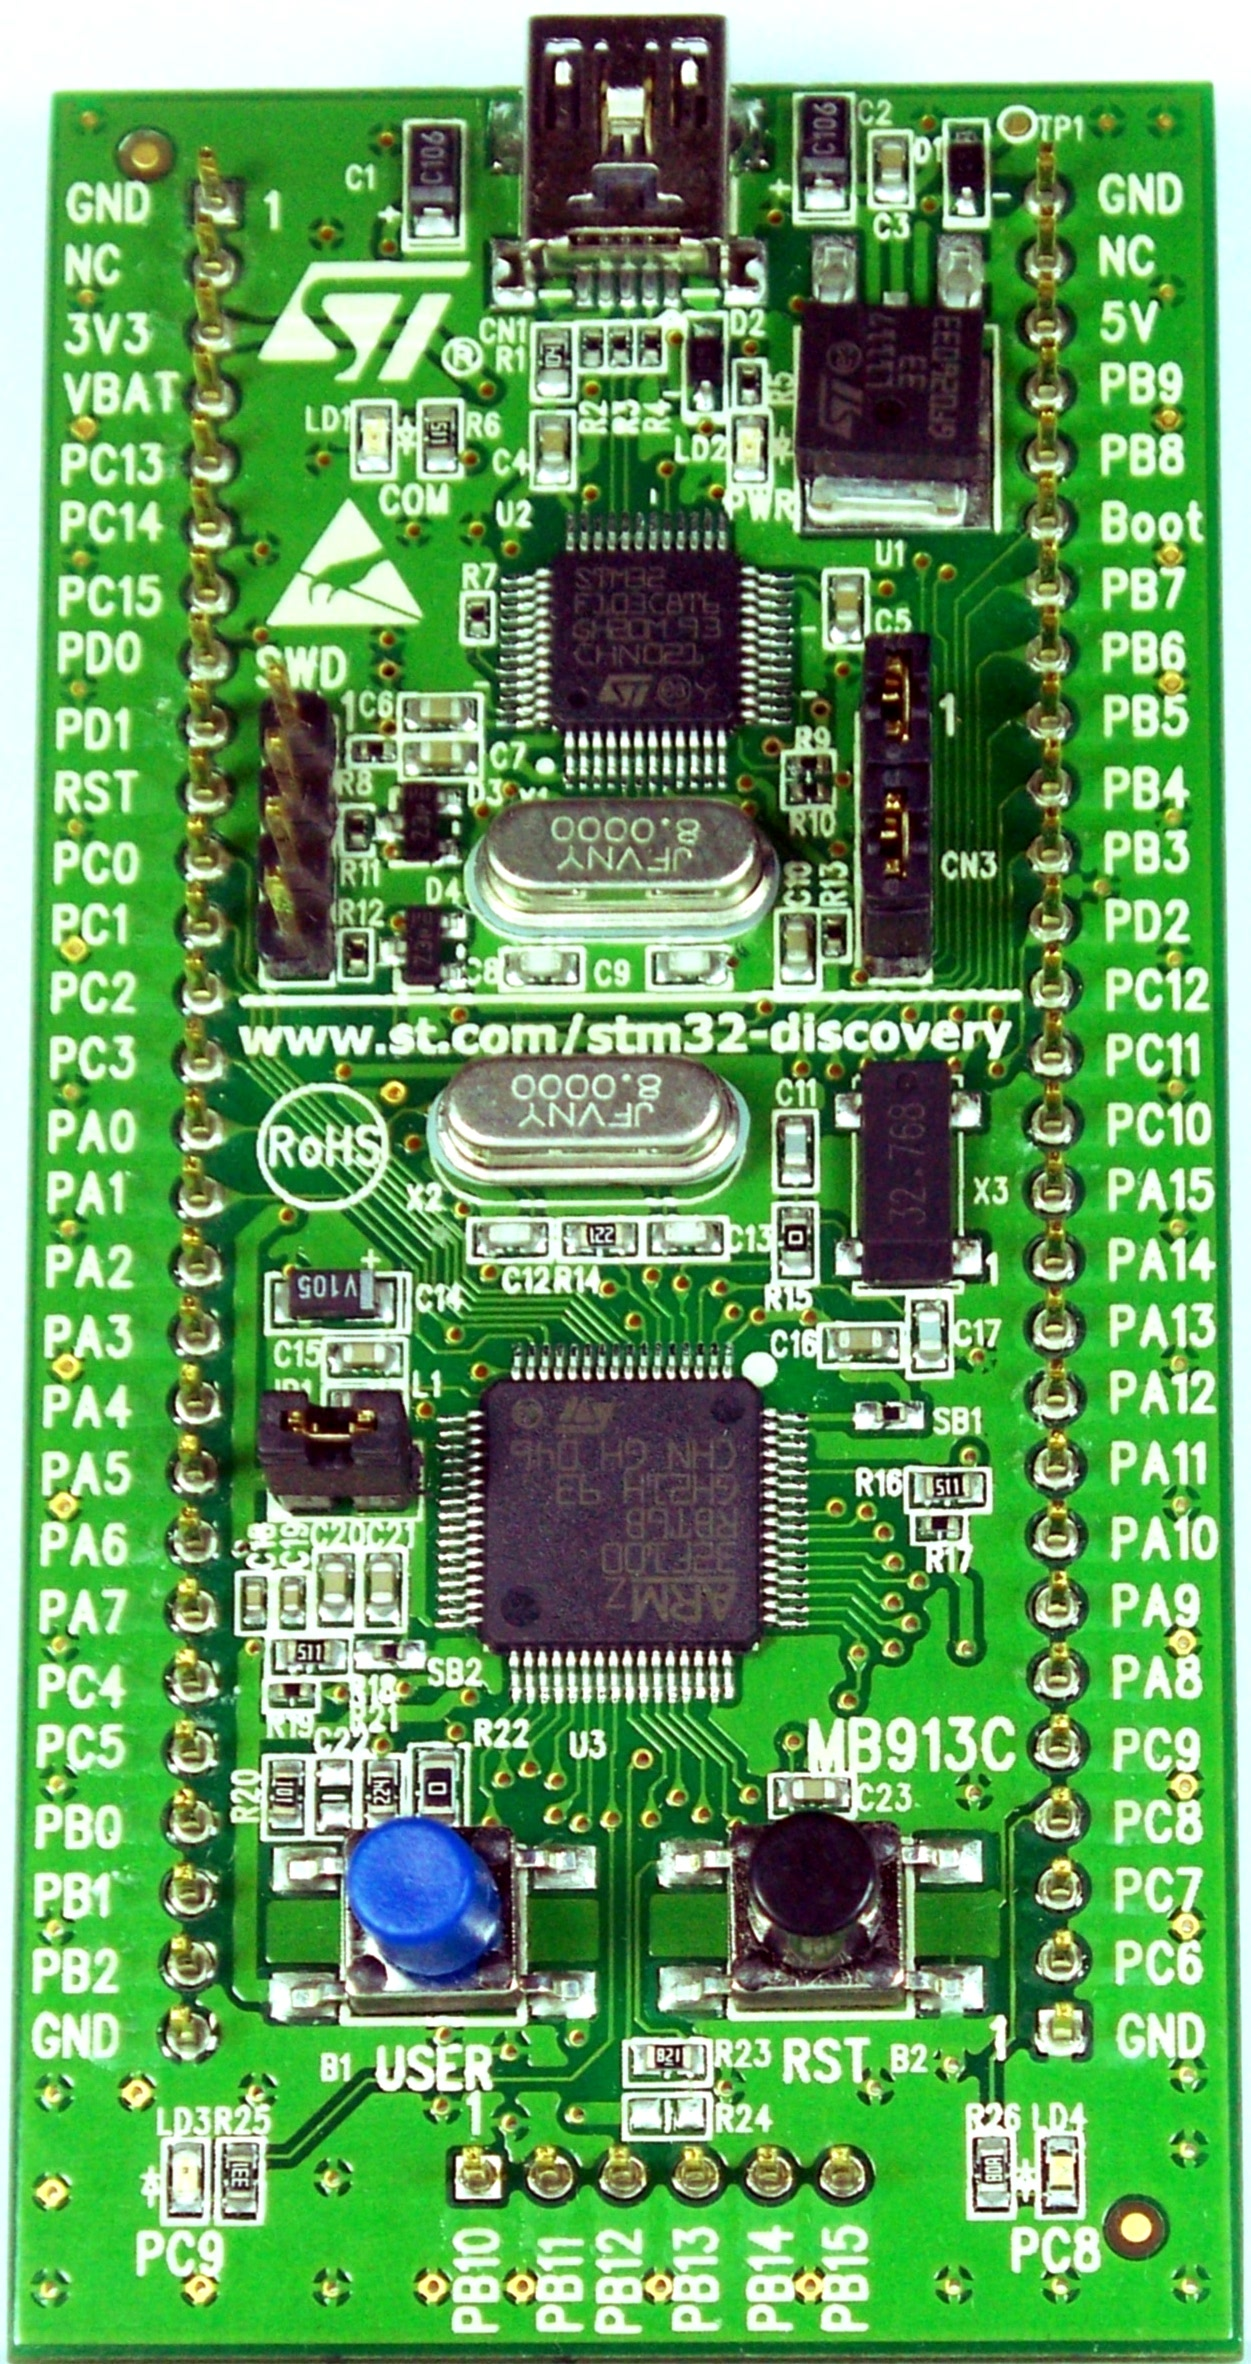
\includegraphics[width=.25\textwidth]{images/stm32_discovery_board.jpg}
\caption{Vývojová doska STM32 vl Discovery}
\label{obr2}
\end{center}
\end{minipage}
\end{center}
\end{figure}

Doska Discovery kit obsahuje len minimum periférií. K dispozícií su dve LED a dve tlačítka (užívateľské a reset). Dobrá vlastnosť je vyvedené programovacie rozhranie na dip lištu. To umožňuje použiť túto dosku na programovanie externe osadených mikrokontrolérov. Veľkou nevýhodou je neprítomnosť UART/USB rozhrania, ktoré by zjednodušilo ladenie. Práve za tým účelom bola navrhnutá testovacia doska. Je vybavená väčšími možnosťami pripojenia periférií. Jedna dutinková lišta je vybavená UART rozhraním aj napájaním. Na toto rozhranie je možné priamo zasunúť prevodník USB/UART s FT232 \cite{usb_uart}. Je potrebné dodržať 3.3V napäťové úrovne. Testovacia doska ďalej obsahuje sadu tlačidiel a LED diód. K dispozícií je aj konektor pre SD kartu. Pre jedoduché ovládanie malých motorov, je na doske prítomný aj mostík, umožňujúci budiť dva motory. Vďaka použitiu low drop stabilizátora je dosku možné napájať aj z jediného li-pol článku. Využitie jeho kapacity však zďaleka nebude najlepšie.

\begin{figure}[ht]
\begin{center}
\begin{minipage}{1.1\linewidth}
\begin{center}
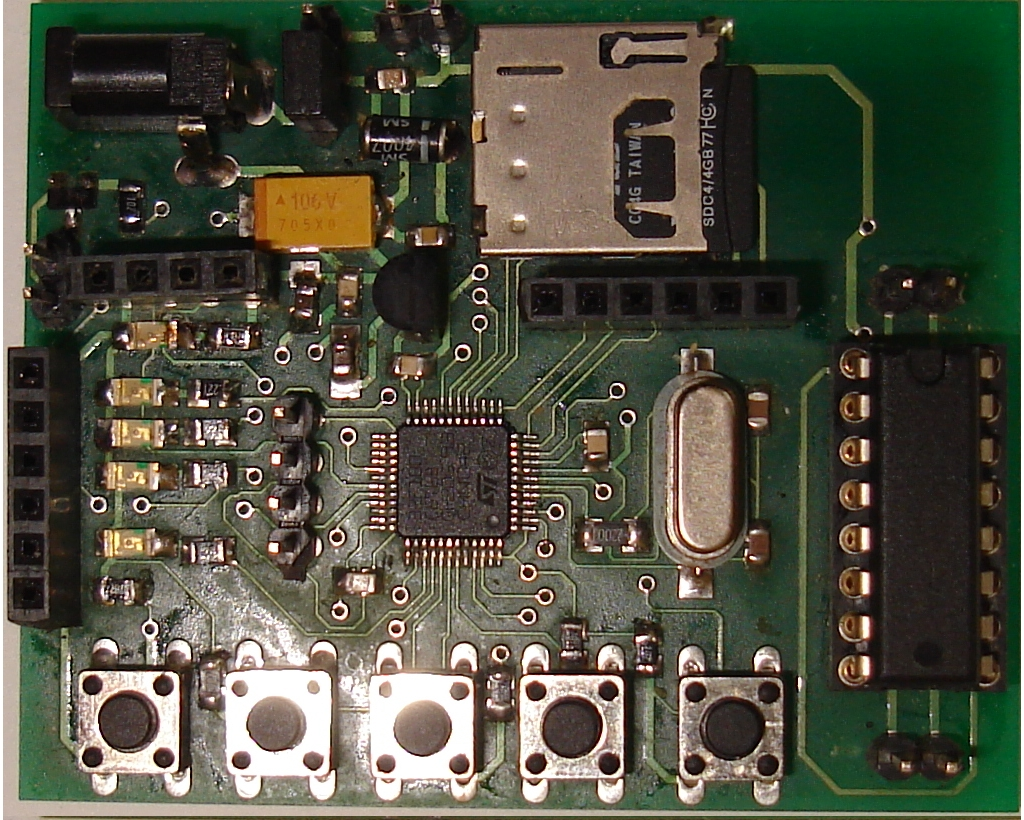
\includegraphics[width=.35\textwidth]{images/test_board.jpg}
\caption{Testovacia doska}
\label{obr2}
\end{center}
\end{minipage}
\end{center}
\end{figure}

\subsection {Stellaris Launchpad}

Pre testovanie funkcionality systému aj na jadre Cortex M4, bola zvolená vývojová doska Stellaris Launchpad firmy Texas Instruments \cite{stellaris_kit}.

\begin{figure}[ht]
\begin{center}
\begin{minipage}{1.1\linewidth}
\begin{center}
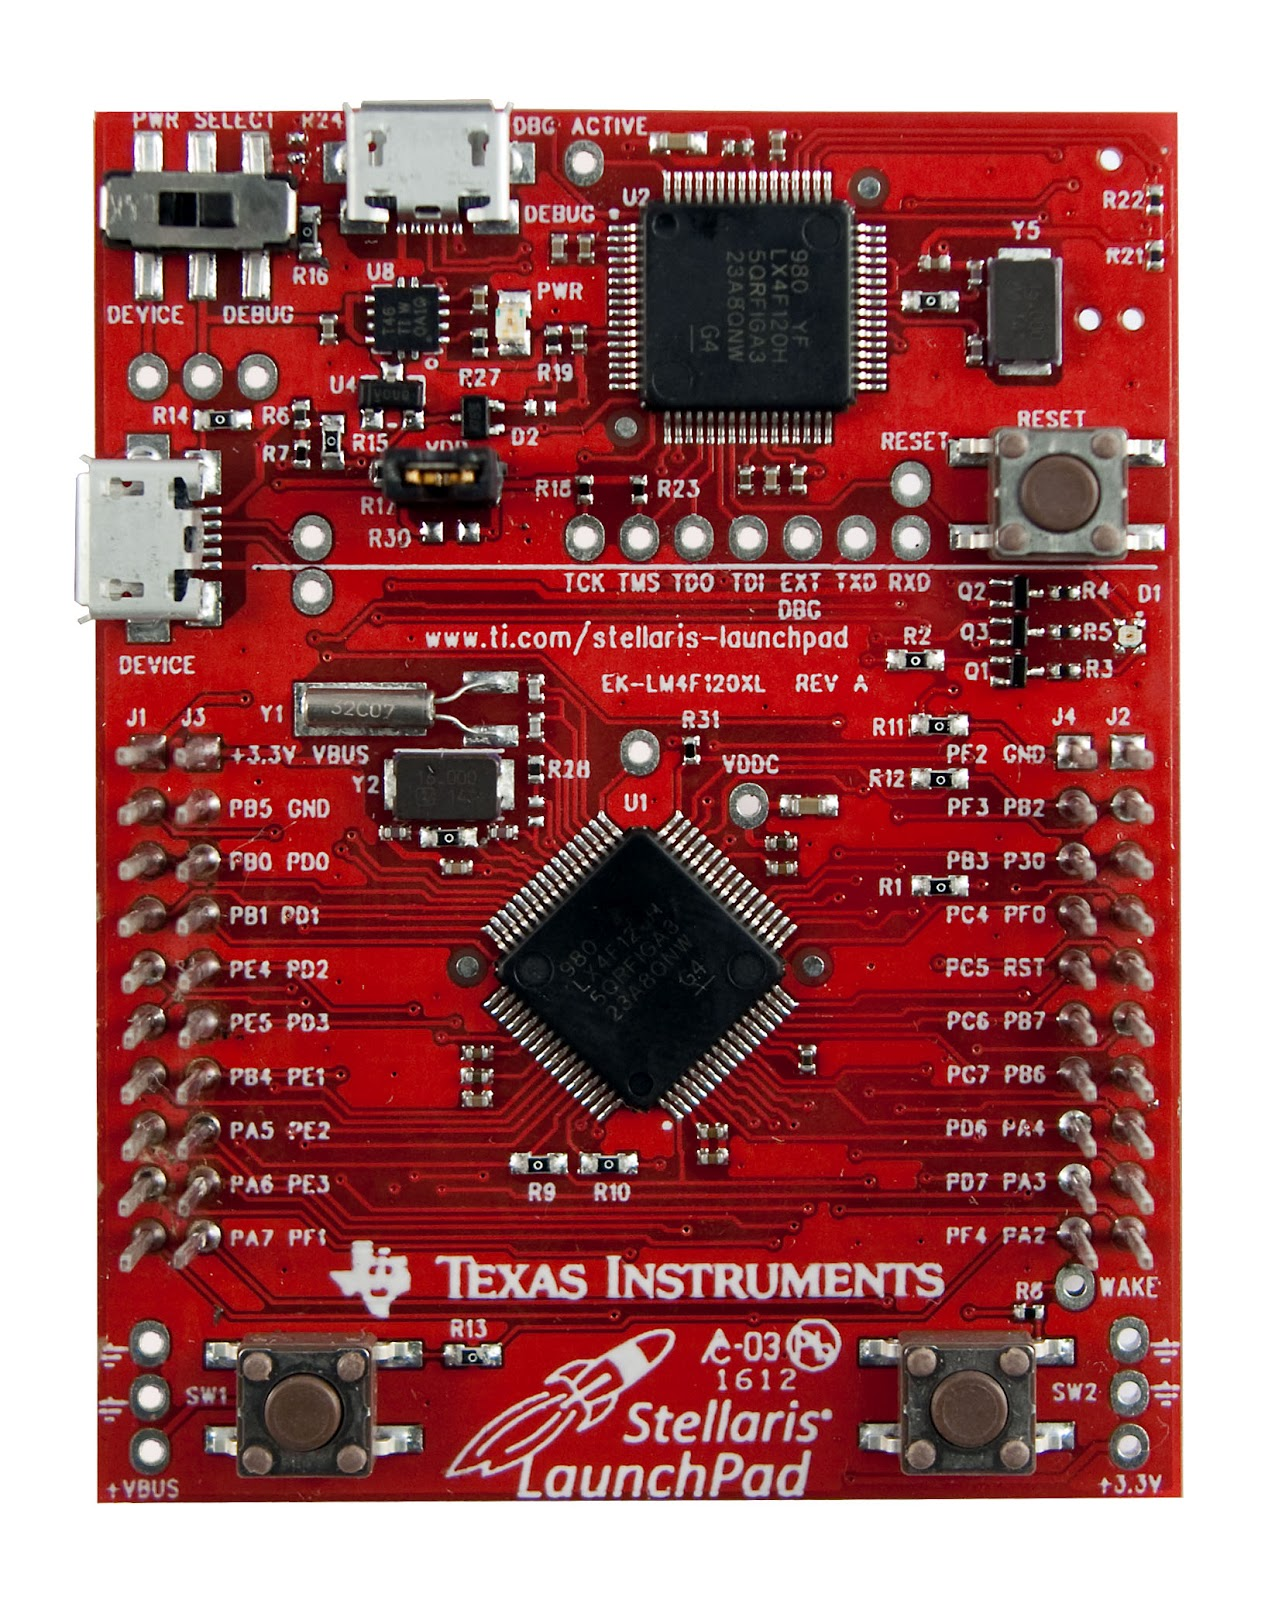
\includegraphics[width=.35\textwidth]{images/launchpad_lm4f120.jpg}
\caption{Vývojová doska Stellaris Launchpad}
\label{obr2}
\end{center}
\end{minipage}
\end{center}
\end{figure}

Doska je vybavená troma tlačidlami. Zaujímavosťou je prítomnosť RGB led diódy. Po pripojení do počítača, sa vytvorí nový sériový port, najčastejšie ako /dev/ttyACM0. Tento fakt veľmi zjednodušuje ladenie aplikácie.

\section {Testovanie jadra}

Na korektné otestovanie jadra je v adresári \textbf{usr/threads} program, ktorý vytvára a ničí vlákna. Tento proces prebieha v cykle a umožňuje tak určit, či sa vlákno správne vytvorí aj ukončí. Dôležitým parametrom je aj čas prepnutia kontextu, z ktorého možno odvodiť záťaž mikroprocesora jadrom systému. Za týmto účelom bol vytvorený dvojvláknový program. Jedno vlákno neustále zapína led. Druhé tú istú led neustále vypína. V obsluhe prerušenia od časovača sa ihneď po uložení kontextu zapne druhá led a tesne pred obnovou kontextu sa led vypne. Pripojením dvojkanálového osciloskopu na dve led, je možné určiť potrebné časy.

\begin{figure}[ht]
\begin{center}
\begin{minipage}{1.1\linewidth}
\begin{center}
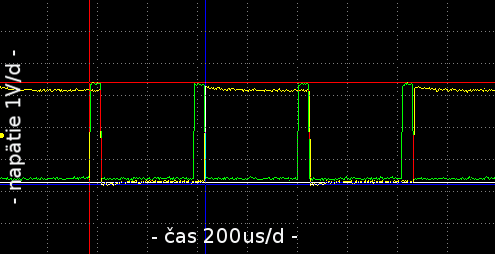
\includegraphics[width=.7\textwidth]{images/cm3_context_switch_02_.png}
\caption{Priebehy napätí pri meraní doby prepnutia kontextu jadra Cortex M3}
\label{obr2}
\end{center}
\end{minipage}
\end{center}
\end{figure}

Frekvencia prepínania kontextu bola zámerne zvýšená na 2kHz, aby sa záznam vošiel na obrazovku. Doba prepnutia kontextu je doba zeleného priebehu. Nameraný čas je 46us pri frekvencií jadra 24MHz. To je približne 1100 inštrukcií (orientačný údaj). 

Pre jadro Cortex M4, taktované na 80MHz bol čas prepnutia kontextu 12us. Pomer rýchosti jadier je 3.33, rovnako ako pomery časov prepnutí kontextu. Merania teda zodpovedajú teoretickému predpokladu - na prepnutie kontextu totiž nie sú využité žiadne špeciálne inštrukcie typické pre jadro Cortex M4.

\begin{figure}[ht]
\begin{center}
\begin{minipage}{1.1\linewidth}
\begin{center}
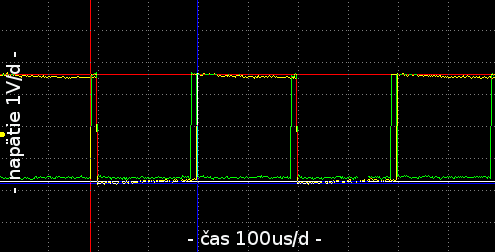
\includegraphics[width=.7\textwidth]{images/cm4_context_switch_02_.png}
\caption{Priebehy napätí pri meraní doby prepnutia kontextu jadra Cortex M4}
\label{obr2}
\end{center}
\end{minipage}
\end{center}
\end{figure}

Treba poznamenať, že vzhľadom na neustále zlepšovanie programu systému, sú súčasné hodnoty už lepšie. Došlo k vyňatiu jedného cyklu, čím sa výrazne znížil potrebný počet inštrukcií a zvýšila efektivita využitia procesora.

\newpage
\section {Testovanie zámkov}

Pre korektné testovanie vstupu a výstupu z kritických sekcií, slúži program \textbf{usr/lock}. Vytvoria sa tri vlákna a každé píše do terminálu svoj text. Funkcia eprint prebieha atomicky. Jednotlivé riadky by teda mali byť zobrazené korektne. V prípade vyhodenia knižnice lock.c, bude text riadkov rozhádzaný a prepletený s inými vláknami. Funguje to vďaka tomu, že UART jednotka je vybavená vyrovnávacou pamäťou a preto znesie náhly nápor dát. Situáciu dobre vystihuje nasledujúci obrázok z terminálového výstupu systému.


\begin{figure}[ht]
\phantom.\hfill
%
\begin{minipage}{0.45\linewidth}
\begin{center}
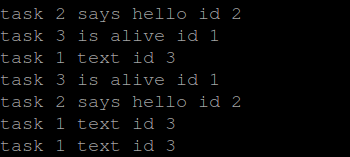
\includegraphics[width=0.9\textwidth]{images/atomic_.png}
\caption{S využitím mutexu}
\label{obrL1}
\end{center}
\end{minipage}
%
\hfill 
%
\begin{minipage}{0.45\linewidth}
\begin{center}
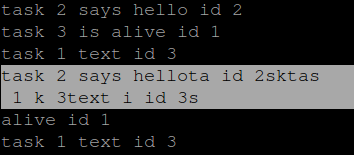
\includegraphics[width=0.9\textwidth]{images/no_atomic_.png}
\caption{Neošetrené použitie}
\label{obrP1}
\end{center}
\end{minipage}
%
\hfill\phantom.
\end{figure}


\section {Testovanie správ}

Systém správ bol testovaný na aplikácií klient-server. Dve vlákna neustále posielajú svoju požiadavku serveru. Požiadavkou bola inkrementácia položky msg.data. Každý klient začal s inou počiatočnou hodnotou. Jeden na 0, druhý na 1. Očakávaný výstup v termináli je potom, že jedon vlákno vypisuje párne a druhé nepárne čísla. Uvedený program je v adresári \textbf{usr/messages}. Pre otestovanie možnosti posielať komplexnejšie dáta, je určená aplikácia cli, v adresári \textbf{usr/cli}. Aplikácia ukazuje prácu so súborovým systémom. Ovládač súborového systému je prítomný ako samostatné vlákno, čakajúce na správu - požiadavka na výpis adresára alebo čítanie súboru. Samotný prenos správy je riešený pomocou pretypovania ukazovateľa a využitia synchrónneho poslania požiadavky serveru.
\newpage
\begin{figure}[ht]
\begin{center}
\begin{minipage}{1.1\linewidth}
\begin{center}
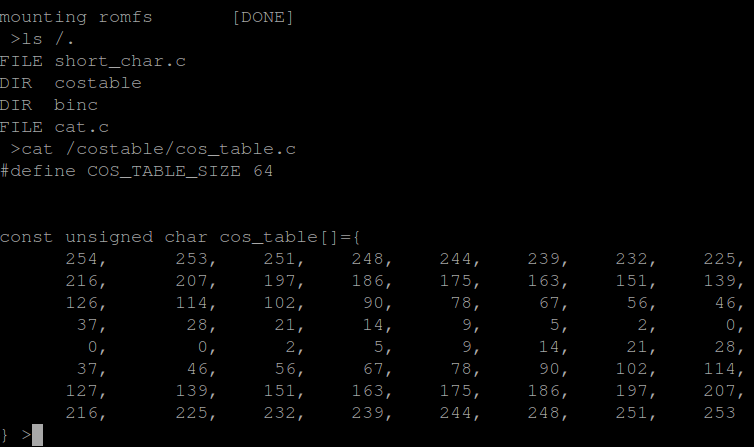
\includegraphics[width=.7\textwidth]{images/romfs_.png}
\caption{Výpis obsahu súboru costable.c}
\label{obr2}
\end{center}
\end{minipage}
\end{center}
\end{figure}

Na obrázku je znázornené použitie súborového systému. Príkazy sú podobné ako v systéme Linux. Treba poznamenať, že primárnym cieľom nebolo vytvorenie komfortného príkazového riadka. Toto rozhranie je implementované najmä za účelmi kvalitného testovania. Ponúkaná funkčnosť je preto veľmi strohá. Implementovať vlastné užívateľské rozhranie však nepredstavuje závažný problém.


